\documentclass [10pt,a4paper]{report}

\usepackage[utf8]{inputenc}
\usepackage{graphicx}
\begin{document}

\part{Le Grid5000}
	\chapter{Présentation du Grid5000}
Le Grid5000 est une grille informatique destiné à la recherche scientifique. Le projet a vu le jour en 2003 et a pour but de promouvoir la recherche sur les grilles informatiques en France. Le Grid5000 est aujourd'hui composé de 1200 noeuds répartis sur 9 sites différents situés en France et au Luxembourg et interconnectés avec le réseau Réseau National de télécommunications pour la Technologie l'Enseignement et la Recherche (RENATER). L'objectif du Grid5000 est de permettre aux scientifiques d'effectuer des expériences dans le domaine des systèmes informatiques et des réseaux distribuées dans un environnement hétèrogene aussi proche de la réalité que possible.

	\begin{figure}[!h]
		\centering
   		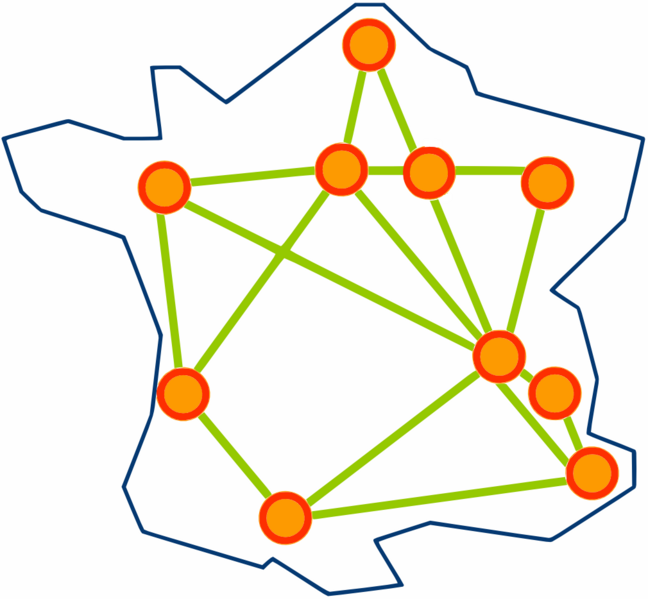
\includegraphics[width=5cm,height=5cm]{map.png}
   		\caption{Localisation des différents sites du Grid5000}
    	\label{fig:map}
	\end{figure} 

Le Grid5000 est donc compsé de plusieurs sites distincts mais l'organisation au sein de chaque site est la même. Chaque site est composé d'un ou plusieurs clusters, c'est à dire un ensemble de machine homogène, par exemple le site de Nancy héberge deux clusters Griffon et Graphene. \\
A l'intérieur de chaque cluster se trouve des ordinateurs aussi appelés "nodes" ou "noeuds". Il existe deux types de nodes : les noeuds de services et les noeuds de travail, sur lesquels sont efectués les expérience. Les noeuds de services servent à l'administration des machines situées dans le cluster et à l'accès aux hôtes virtuels pour les administrateurs. Certains noeuds de services appelés "frontends" sont utilisés par les utilisateurs pour l'accès aux différents sites grâce au protocole ssh, la réservation de noeuds et le déploiment. 

\begin{figure}[!h]
		\centering
   		\includegraphics[width=5cm,height=5cm]{griffon.jpeg}
   		\caption{Un des clusters de Nancy : Griffon}
    	\label{fig:griffon}
	\end{figure}
	
	\chapter{Les outils du Grid5000}
		Le Grid5000 est composé de plusieurs services: une partie ces services ont été développés uniquement pour ce projet comme par exemple Kadeploy3 qui a été developpé par l'INRIA Nancy - Grand Est; les autres sont des serivces standard déjà utilisés sur les systèmes Unix.  
		\section{OAR2}			
			OAR est un gestionnaire de ressources (batch scheduler) pour grandes grappes de calcul. Il est écrit en scripts PERL articulé autour d’une base SQL (Postgres ou MySQL). Il est composé de modules indépendants qui interagissent via la base de données.
		\section{Kadeploy3}
		\section{Taktuk}
			Taktuk est un outils complémentaire à OAR2. Taktuk permet l'éxecution de commande à distance sur un grand nombre de noeuds hétérogènes.
		\section{KaVLAN}
			KaVLAN est un outils qui a pour but de permettre de mettre en place un VLAN sur des noeuds du Grid5000. Il permet la mise en place de plusieurs type de VLAN : local, "router" et global. KaVLAN peut être utiliser en complément de Kadeploy et de OAR pour certains types d'expérimentation.\\
			\begin{itemize}
  				\item Un KaVLAN local est un VLAN completement isolé du reste de la plateforme Grid5000. Il est alors obligatoirement d'utiliser une gateway pour accéder aux noeuds se trouvant à l'intérieur de VLAN.
  				\item Un KaVLAN "router" permet l'accès à tous les noeuds du VLAN depuis le reste du Grid5000 sans utiliser de gateway.
 				 \item Un KaVLAN global est un VLAN qui est disponible sur tous les sites du Grid5000. Un routeur est alors configuer sur le site où le VLAN a été configuré.
			\end{itemize}
			
		\section{Les autres outils}
	
\end{document}
